\documentclass[a4paper,twoside]{report}
\usepackage{graphicx}
\usepackage{dsfont}
\usepackage{amsfonts}
\usepackage{epsf,amsthm,amsmath}
\usepackage[ngerman]{babel}
\usepackage[latin1]{inputenc}
\usepackage{graphicx}
\setlength{\parskip}{5pt plus 8pt minus 2pt}
\pagestyle{headings}

\begin{document}
\begin{titlepage}
\ \vfill
\Large
\begin{center}
{\LARGE\bf Proseminar} \\[1cm]
{\huge\bf Stochastische Dynamische Optimierung\par}
\vspace*{1cm}
\input unilogo
\unilogo{30}\\[1cm]
{\bf Universit"at Karlsruhe (TH)}\\
{Fakult"at f"ur Mathematik}\\
{\em Institut f"ur Mathematische Stochastik}
\vfill
Priv.-Doz.~Dr.~D.~Kadelka\\
Dr.~B.~Klar
\vfill\vfill 
Sommersemester 2004
\vfill
\vfill
\end{center}
\end{titlepage} 
\thispagestyle{empty}
\ 
\vfill
\noindent
Copyright $\copyright$ 2004\\
Institut f"ur Mathematische Stochastik\\
Fakult"at f"ur Mathematik\\
Universit"at Karlsruhe\\
Englerstra"se 2\\
76\,128 Karlsruhe


\title{Stochastic Scheduling}
\author{Clemens Lode}
\date{}
\maketitle

\pagenumbering{roman}
\tableofcontents

\pagenumbering{arabic}

\setcounter{chapter}{2}
\chapter{Stochastic scheduling}
\section{Einleitung}

\textsc{Stochastic Scheduling} besch"aftigt sich mit Problemen, bei denen die Laufzeiten eines Jobs durch Zufallsvariablen dargestellt sind. Dadurch ist die tats"achliche Zeit vor Ende des Jobs unbekannt. Das 'Scheduling' ist je nach Problem auf ein oder mehrere Prozessoren und mit verschiedenartigen Nebenbedingungen best"uckt.

Hier im Speziellen m"ochte ich auf vier F"alle aus diesem Bereich eingehen die mit der Abarbeitung von Jobs auf ein oder mehreren Prozessoren zu tun haben.

\section{Fall: Ein Prozessor}

Zum Einstieg ein triviales Problem um mit den verwendeten Variablen und ein paar einfachen Gesetzm"assigkeiten im weiteren Verlauf besser zurechtzukommen. 
Das Problem in diesem Fall ist, dass wir \emph{n} Jobs auszuf"uhren haben. Ein Job ist dabei eine beliebige Aufgabe die ein Prozessor berechnen kann, der eine bestimmte Zeit braucht, wobei die Jobs nicht gleich sein m"ussen.
Au"serdem haben wir im ersten Fall einen einzelnen Prozessor zur Verf"ugung, der immer nur einen Job gleichzeitig bearbeiten kann. Die Fragestellung ist nun, welche Reihenfolge der Jobs, im Folgenden Politik genannt, die Zeit um alle Jobs auszuf"uhren minimiert.

Was ist die ben"otigte Gesamtzeit unserer Jobs? Bei einem realistischen Beispiel w"are das schwer zu sagen. Verbraucht z.B. ein Job w"ahrend und nach der Bearbeitung sehr viel Speicher w"are wohl das Beste diesen hinten hinzustellen, damit die anderen Jobs nicht z.B. auf der langsamen Festplatte ausgelagert werden m"ussen. Die Zeit die ein einzelner Job ben"otigt w"are also vom bisherigen Verlauf abh"angig.

Wir machen es uns jedoch einfach und begrenzen uns auf den Fall, dass \emph{alle Jobs unabh"angig voneinander} bearbeitet werden k"onnen. Dies bedeutet in diesem Fall, dass zu jedem Zeitpunkt auf Basis der bisherigen Ereignisse die bedingte Wahrscheinlichkeit fuer jeden neuen Job eine bestimmte Zeit zu brauchen genau so gro"s ist, als w"are dies der erste Job in der Auftragsliste.

Im Weiteren werde ich folgende Definitionen und Voraussetzungen gebrauchen:
\begin{itemize}
\item M: ben"otigte Gesamtzeit bis alle Jobs abgearbeitet sind
\item Politik \begin{displaymath}\pi = (i_{1},i_{2},\ldots,i_{n})\end{displaymath} wobei \(i_{j}\) \(\neq\) \(i_{k}\) f"ur \(j \neq k\) und \(0<i_{j}\le n\) eine Jobnummer bezeichnet.
\item \(X_{j}\) ist eine Zufallsvariable mit Exponentialverteilung mit Parameter \(\lambda_{j}\)
\end{itemize}

Die Gesamtzeit unserer Jobs ist dann nat"urlich die Summe aller Zeiten und somit von der Reihenfolge unabh"angig. Also ist es, wie man es erwartet h"atte, vollkommen egal, welche Politik man w"ahlt. F"ur die erwartete Gesamtzeit ergibt sich also:

\begin{displaymath} E(M) = E(X_{i_{1}})+E(X_{i_{2}})+\cdots+E(X_{i_{n}}) = \sum_{j=1}^{n} E(X_{j})\end{displaymath}

wobei die Summe unabh"angig von den \(i_{j}\), also der Reihenfolge der Jobs, ist.

\begin{figure}[h]
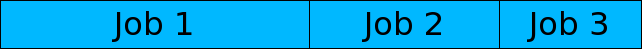
\includegraphics[scale=0.5]{durchlaufpolitik1.png}
\caption{M"oglicher Durchlauf bei gegebener Politik \(\pi_{1} = (1,2,3)\)}
\end{figure}

\begin{figure}[h]
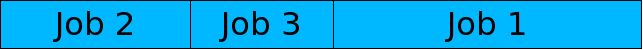
\includegraphics[scale=0.5]{durchlaufpolitik2.png}
\caption{Der selbe Durchlauf mit anderer Politik \(\pi_{2} = (2,3,1)\)}
\end{figure}

Mit dieser kleinen Einf"uhrung k"onnen wir uns nun an ein schwierigeres Problem wagen, wir legen im zweiten Teil einen weiteren Prozessor hinzu.

\newpage\section{Fall: Zwei Prozessoren parallel}

\subsection{Problemdefinition und Ansatz}

Es sind wieder eine Reihe von Jobs gegeben, die unterschiedlich lange Zeit ben"otigen. Au"serdem hat man ein System mit diesmal zwei identische Prozessoren zur Verf"ugung. Die einzelnen Jobs sind stochastisch unabh"angig und exponential verteilt. Das Problem ist nun wieder, eine Politik f"ur die Abarbeitung der Jobs zu finden, so dass die insgesamt ben"otigte Zeit minimal ist.

\begin{figure}[h]
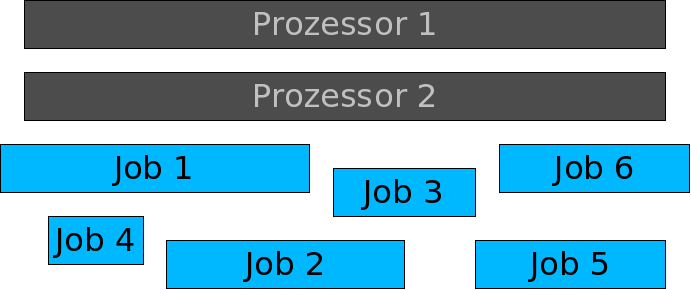
\includegraphics[scale=0.5]{zweiprozessoren.png}
\caption{"Ubersicht Problemstellung zwei Prozessoren - mehrere Jobs m"ussen auf zwei Prozessoren verteilt werden}
\end{figure}

Ein erster Ansatz w"are, die Politiken so aufzubauen, dass wir jedem Job \emph{j} einen Zeitpunkt \emph{k} und einen Prozessor \emph{l} zuordnen. Zwar sind damit alle m"oglichen Kombinationen abgedeckt, jedoch ergibt sich beim Zeitpunkt \emph{k} ein Problem: Es ergeben sich einerseits Zeiten in der Prozessoren ungenutzt sind (siehe Abb. 3.4), die deshalb auftreten, weil die Ausf"uhrungszeiten \(X_{j}\) der Jobs zu Beginn unbekannt sind. Andererseits gibt es keine festen Zeiteinheiten auf die wir unsere Jobs verteilen k"onnten was zu unendlich vielen M"oglichkeiten f"uhren w"urde. Vor allem auf Grund der ungenutzten Zeiten bei dieser Art von Politik kann in diesem Fall die optimale L"osung f"ur die gegebenen Voraussetzungen nicht gefunden werden.

\begin{figure}[h]
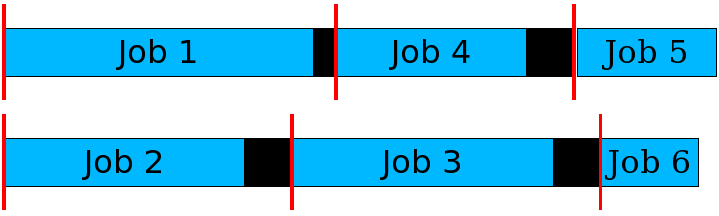
\includegraphics[scale=0.5]{zeitzuordnung2.png}
\caption{Zustand Prozessoren mit Politik die nach Zeit zuordnet - schwarz markierte Bereiche geben ungenutzte Zeiten des Prozessors an}
\end{figure}


\subsection{Benutzung von Expertenwissen und Onlineregeln}

Die Einteilung nach den Zeitpunkten k"onnen wir umgehen indem wir eine Voraussetzung, sogenanntes \emph{Expertenwissen}, f"ur unser Problem benutzen. Wir m"ussen n"amlich "uber die genaue Positionen der Jobs zu Beginn noch nichts wissen, wir k"onnen uns entscheiden welchen Job wir als n"achstes einf"ugen sobald einer der beiden Prozessoren frei wird. Wir d"urfen also durch diese Onlineregel die Jobs nahtlos aneinander anf"ugen, was zur Schlie"sung der L"ucken f"uhrt. Intuitiv ist klar, dass wir dadurch auch die optimale L"osung erreichen k"onnen, da wir nun die M"oglichkeit haben, die Jobs so in die Prozessoren einzuf"ugen, dass der Abstand beider 'Jobs"aulen', also \emph{D} minimal wird. Ein genauer mehrseitiger Beweis, dass Politiken die den Prozessor zu keiner Zeit (au"ser am Ende) unbesch"aftigt lassen nicht optimal sind, ist in der Literatur (z.B. f"ur den Fall der Tandemschaltung [3]) finden.

Der zweite Versuch eine Politik aufzustellen, w"are also, dass man jeden Job in eine der zwei Prozessoren in einer bestimmten Reihenfolge einf"ugt. Wir ordnen jedem der \emph{n} Jobs einen Prozessor zu (\(2^{n}\) M"oglichkeiten) und legen die Reihenfolge der \emph{n} Jobs fest (\(n \cdot (n-1) \cdots 2 \cdot 1 = n!\) M"oglichkeiten) wodurch sich insgesamt \(2^{n} n!\) Belegungen f"ur die Politik ergibt. 

Da man dabei mehrere Politiken erh"alt, die eine gleiche Belegung der Jobs auf die Prozessoren zur Folge hat (z.B. 3 und 4 auf Prozessor 1, 1 und 2 auf Prozessor 2 \(\Rightarrow\) 1, 2, 3, 4 f"uhrt zur selben Belegung wie 3, 4, 1, 2) ist die Zahl der unterschiedlichen Politiken geringer. Wir k"onnen k Jobs auf einen und \((n-k)\) Jobs auf den anderen Prozessor legen und dann \(n!\) bzw. \((n-k)!\) verschiedene Reihenfolgen \(A\)aufstellen:		
		
\begin{displaymath}\sum_{k=0}^{n} \sum_{A:|A|=k} k!(n-k)! = \sum_{k=0}^{n}{n \choose k} k!(n-k)! = \sum_{k=0}^{n}n!\end{displaymath}
\begin{displaymath}= (n+1)!\end{displaymath}

\subsection{Aufstellung der zu minimierenden Zielfunktion}

Seien zwei identische Prozessoren gegeben um \emph{n} Jobs abzuarbeiten. Beide laufen unabh"angig, k"onnen also jede Aufgabe zu jeder Zeit in einer beliebigen Reihenfolge bearbeiten. Startzeit ist \(t = 0\). 

F"ur jede Politik \(\pi\) ist jeweils \emph{M} die Bearbeitungsdauer und \emph{D} die Zeit die einer der Prozessoren stillsteht. Somit ist zum Zeitpunkt \(M - D\) einer der Prozessoren fertig und keine weiteren Auftr"age mehr in der Warteschlange und \(M + M - D\) ist die Summe aller Zeiten, also \(\sum_{j=0}^n X_{j}\)

Also gilt: \(2M - D - \sum_{j=0}^{n} X_{j} = 0\) und somit f"ur jede Politik \(\pi\):

\begin{displaymath}E_{\pi}(2M-D-\sum_{j=0}^{n} X_{j}) = E_{\pi}(0)\end{displaymath}

\begin{displaymath}2 E_{\pi} (M) = E_{\pi} (D) + \sum_{j=0}^{n} E_{\pi} (X_{j})\end{displaymath}

Da nach Voraussetzung die \(X_{j}\) von einander also insbesondere auch von der Wahl der Politik \(\pi\), unabh"angig sind, ist \(\sum_{j=0}^{n} E(X_{j})\) eine Konstante f"ur jede Politik \(\pi\) (f"ur die gleichen \(X_{j}\)) und wir setzen \(c = \sum_{j=0}^{n} E(X_{j})\):

\begin{equation}\label{e31}E_{\pi}(M) = \frac{E_{\pi}(D) + c}{2}\end{equation}

Also ergibt sich, dass durch \emph{Minimierung der erwarteten Differenz D} in der einer der Prozessoren unbesch"aftigt ist, auch die Bearbeitungsdauer minimiert wird.

\subsection{Verfeinerung der Politik}
	
Zwar k"onnte man unter Umst"anden auch mit dem Modell jedem Job einen Prozessor zuzuordnen auf die einzelnen Aussagen und S"atze kommen, jedoch ist es bei Optimierungsaufgaben grunds"atzlich hilfreich, die Zahl der unterschiedlichen Politiken so weit wie m"oglich zu verringern. Dabei ist nat"urlich immer darauf zu achten, dass der optimale Fall mit der Politik noch herzustellen ist.

Im Weiteren wird ausgenutzt, dass wir eben keine station"are Entscheidung vor Beginn des Einf"ugens treffen m"ussen, sondern w"ahrend des Laufs in jedem Moment eingreifen k"onnen. Dass dies nur sinnvoll ist, wenn gerade ein Job beendet wurde bzw. ein Prozessor frei ist, wurde im vorherigen Abschnitt gezeigt. Dass es auch m"oglich ist, die Zuweisungen einzelner Jobs zu den Prozessoren zu Beginn wegfallen zu lassen, wird im Folgenden gezeigt.

\textbf{Behauptung}: Eine Politik die die Jobs nach ihrer Reihenfolge immer auf den Prozessor legt, der gerade frei ist, ist gleichwertig mit einer Politik die zu Beginn jedem Job einen Prozessor zuweist und auf die jeweiligen Prozessoren entsprechend nach der Reihenfolge legt.

Mit ''gleichwertig'' ist hier gemeint, dass mit beiden Politiken die Jobs so verteilt werden k"onnen, dass die insgesamte ben"otigte Zeit bei beiden Politiken gleich und minimal ist, dass also vor allem der optimale Fall nicht wegf"allt

\textbf{Beweisidee}: Es ist klar, dass der Versuch auf den einen Prozessor alle Jobs und auf den anderen Prozessor keine Jobs zu verteilen f"ur \(n>1\) nicht zum optimalen Ergebnis f"uhrt, da die erwartete Differenz \emph{D} in dem Fall maximal w"are. 
So eine 'kaputte' Politik k"onnte man aber 'reparieren' in dem man, zu jedem Zeitpunkt zu dem beiden Prozessoren keine Aufgabe zu bearbeiten hat, einfach die n"achste Aufgabe aus unserer Politik zuweist. Jede Politik die mit der Konstruktionsmethode aus der Behauptung nicht hergestellt werden kann, kann keine optimale Politik sein, da dies bedeuten w"urde, dass am Ende zwei Politiken hintereinander gesetzt werden, obwohl zum Ende des vorletzten Jobs der andere Prozessor frei ist. Dagegen h"atte ein fr"uheres Verschieben des letzten Jobs auf den unbesch"aftigten Prozessor eine Verbesserung zur Folge.

Wenden wir diese Regel auf jede unserer Politiken an, folgt, dass eine Politik die alle \emph{n} Jobs auf einen Prozessor legt, \emph{gleichwertig} zu allen anderen Kombinationen der Verteilung der Jobs ist.
\begin{figure}[h]
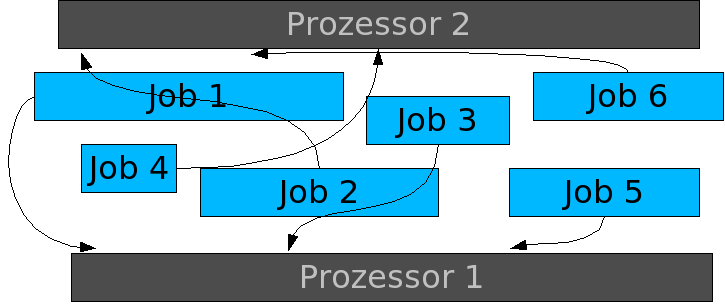
\includegraphics[scale=0.5]{zweiprozpfeile.png}
\caption{Zwei Prozessoren - eine Politik}
\end{figure}

Dies reduziert unseren Zahl unterschiedlicher Politiken auf \textbf{n!} und erleichtert die folgenden Beweise, da wir nur noch Politiken haben die die Jobs der Reihenfolge nach anordnen, anstatt noch jedem Job einen Prozessor zuzuordnen.

\emph{Bemerkung:} Diese Politik ist zwar f"ur sich gesehen station"ar, jedoch nicht die daraus resultierende Verteilung der Jobs auf die Prozessoren, da wir w"ahrend der Bearbeitung noch mit der Regel 'Lege Job auf einen unbesch"aftigten Prozessor' die Reihenfolge anpassen. 

Die Frage ist nun, ob durch unsere Regel das Problem nicht schon gel"ost wurde. Wenn wir immer eine Aufgabe auf den Prozessor legen, der nicht besch"aftigt ist, gleichen wir bei jedem Schritt beide Balken aus. Erreichen wir dadurch das optimale Gleichgewicht? Nein. Dies w"urde der Fall sein, wenn alle Jobs gleiche Zeit ben"otigten und eine gerade Anzahl Jobs vorliegt, also auf jeden Prozessor gleich viele Jobs gelegt werden k"onnen und somit auch \emph{D} minimal w"are. Legen wir aber beispielsweise die Jobs mit absteigenden \(\lambda_{i}\) ( = aufsteigenden erwartete Zeiten) auf die Prozessoren, schwankt der Unterschied \emph{D} zwischen beiden bei jedem weiteren Schritt mehr:
	
\begin{tabular}{|r|ccc|}
\hline
Schritt & Idle-Zeit & 1. Prozessor & 2. Prozessor \\
\hline
0 & 1 & 1 & 0 \\
1 & 1 & 1 & 2 \\
2 & 2 & 4 & 2 \\
3 & 2 & 4 & 6 \\
4 & 3 & 9 & 6 \\
5 & 3 & 9 & 12 \\
... & ... & ... & ... \\
\hline
\end{tabular}

Investiert man in die Aufgabe etwas Denkarbeit wird auch klar, dass wohl die optimale Politik w"are, wenn wir grunds"atzlich mit den l"angsten Jobs beginnen und am Schluss die k"urzesten Jobs legen. Warum? Weil wir bei jedem Schritt die Aufgabe grunds"atzlich nur auf den Prozessor legen, der gerade frei ist. Wir versuchen also bereits dadurch die beiden Balken auszugleichen. Je sp"ater wir eine l"angere Aufgabe auf einen Prozessor legen, desto unwahrscheinlicher k"onnen wir diesen mit den restlichen Jobs wieder ausgleichen. Dies bleibt nun noch formal zu zeigen.

\subsection{Erster Beweisschritt: Vergleich zweier Politiken}

Sei im weiteren Verlauf zu Begin bereits ein Job \emph{0} bereits im Prozessor, d.h. starte jede Politik mit Job \emph{0} (dies macht den Beweis etwas klarer).

Als n"achstes wird gezeigt, dass eine Politik die in aufsteigender Reihenfolge der \(\lambda_{i}\) (also der absteigenden erwarteten Bearbeitungszeiten) angeordnet ist, optimal ist. Dazu betrachten wir zuerst zwei nahezu gleiche Politiken, bei denen Job \emph{1} und Job \emph{2} miteinander vertauscht sind und beweisen dann induktiv:

\textbf{Lemma 1:} Seien zwei Politiken \(\pi\) und \(\bar \pi\) gegeben:
\begin{displaymath}\pi = (0,2,1, i_{3}, i_{4},\ldots,i_{n})\end{displaymath} 
\begin{displaymath}\bar \pi = (0, 1,2,i_{3}, i_{4},\ldots,i_{n})\end{displaymath} 
Gelte au"serdem, dass \(\lambda_{1} = min_{k \ge 1}(\lambda_{k})\), dann gilt:
\begin{displaymath}E_{\bar \pi}(D)\le E_{\pi}(D)\end{displaymath}


\textbf{Beweis:} Seien \(p_{j}\) und \(\bar p_{j}\), \(j \ge 0\) die zu \(\pi\) und \(\bar\pi\) geh"origen Wahrscheinlichkeiten, dass die letzte von den Prozessoren abgeschlossene Aufgabe Job \emph{j} ist, also z.B. Prozessor \emph{1} fertig ist und Prozessor \emph{2} noch an Aufgabe \emph{j} arbeitet und keine weiteren Jobs mehr in der Warteschlange/Politik liegen.

\begin{displaymath}p_{0} = \bar p_{0} = \mathbb{P}(X_{0} > \sum_{j=1}^{n} X_{j})\end{displaymath} ist klar. Der erste Job entspricht der Wahrscheinlichkeit, dass \(X_{0}\) gr"osser ist als alle anderen zusammengenommen, da \(p_{0}\) ja jeweils der erste Job in beiden Politiken \(\pi\) und \(\bar \pi\) ist.

Wir wollen nun durch Induktion zeigen, dass \begin{equation}\label{e32}\bar p_{1} \le p_{1}, \qquad \bar p_{j} \ge p_{j}, \qquad  j=2,\ldots,n\end{equation}

\textbf{Induktionsanfang:} F"ur \(n = 1\) f"allt \(\bar p_{j} \ge p_{j}\) f"ur \(j = 2,\ldots,n\) sowieso weg, da \(n < 2\) und \(\bar p_{1} \le p_{1}\) gilt nach der Voraussetzung \(\lambda_{1}\) = \(min_{k \ge 1}(\lambda_{k})\), da \(\pi\) an der Stelle 1 \(\lambda_{1}\) stehen hat und \(\bar \pi\) dagegen \(\lambda_{2}\).

\textbf{Induktionsvoraussetzung:} Es gelte also die Behauptung (\ref{e32}) f"ur den Fall, dass nur n-1 Jobs (zus"atzlich zu Job 0) vorliegen und somit:
\begin{equation}\label{e33}\bar p_{1}^{*} \le  p_{1}^{*}, \qquad \bar p_{j}^{*} \ge  p_{j}^{*}, \qquad  j=2,\ldots,n-1\end{equation}

\textbf{Induktionsschluss:} Seien nun diesmal \((n-1)+1 = n\) Jobs zu erledigen und seien \( p_{j}^{*}\) und \(\bar p_{j}^{*}\) (wieder zugeh"orig zu \(\pi\) und \(\bar\pi, j=1,\ldots,n-1\) die Wahrscheinlichkeiten, dass Job \emph{j} der letzte der Jobs \(0,\ldots,n-1\) f"ur die jeweilige Politik ist.
Da die Jobs unab"angig sind, k"onnen wir zur Betrachtung des letzten Jobs alle vorherigen abgeschlossenen Jobs ignorieren, diese haben keine Auswirkung auf die Bearbeitungszeit f"ur den letzten Job. Allerdings liegt unter Umst"anden auf dem anderen Prozessor noch ein letzter Job \emph{n} der zu Beginn des letzten Jobs noch nicht abgeschlossen ist. 
Nach der Ged"achtnislosigkeit der Jobs, die aus der Exponentialverteilung folgt, l"auft dieser Job \emph{n} noch \(X_n\) Zeiteinheiten obwohl er schon einige Zeit gelaufen ist, genauer gesagt bleibt die Verteilung der Lebensdauer eines Jobs, der \emph{s} Einheiten gelaufen ist, dieselbe ist wie die eines neuen Jobs. Dies k�nnen wir schreiben in der Form:
\begin{displaymath}\mathbb{P}(X>s+t|X>s)=\mathbb{P}(X>t)\end{displaymath}

\begin{figure}[h]
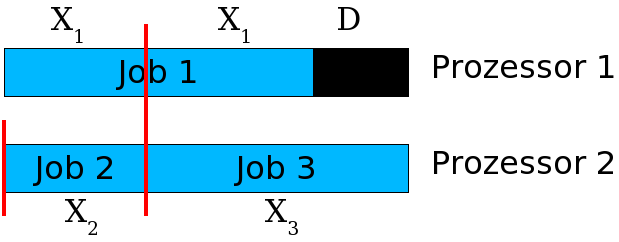
\includegraphics[scale=0.5]{gedaechtnis.png}
\caption{Abschneiden unter Ausnutzung der Ged"achtnislosigkeit - Kein Einfluss auf \(X_{1}\)}
\end{figure}

Daraus folgt, dass die Wahrscheinlichkeit, dass Job \emph{j} und nicht Job \emph{n} der letzte bearbeitete Job ist, \(\mathbb{P}(X_{j} > X_{n})\) entspricht:

\begin{displaymath}\mathbb{P}(X_{j} > X_{n}) = \int_{x=0}^{\infty} \mathbb{P}(X_{n} < x | X_{j} = x) f(x,\lambda_{j}) dx = \int_{0}^{\infty}(1 - e^{-\lambda_{j}x})\lambda_{j}e^{-\lambda_{n}x} dx\end{displaymath}
\begin{displaymath}= \int_{0}^{\infty} (\lambda_{j}e^{-\lambda_{j}x} - \lambda_{j}e^{(-\lambda_{n}-\lambda_{j})x})dx = [-e^{-\lambda_{j}x} + \frac{\lambda_{j}}{\lambda_{j}+\lambda_{n}} e^{(-\lambda_{n} - \lambda_{j})x}]_{0}^{\infty}\end{displaymath}
\begin{displaymath}= 1 - \frac{\lambda_{j}} {\lambda_{j} + \lambda_{n}} = \frac{\lambda_{j} + \lambda_{n} - \lambda_{j}}{\lambda_{j} + \lambda_{n}}\end{displaymath}
\begin{displaymath}= \frac{\lambda_{n}}{\lambda_{n} + \lambda_{j}}\end{displaymath}

Da diese Wahrscheinlichkeit unabh"angig von der Wahrscheinlichkeit ist, dass \emph{j} im Fall mit insgesamt \(n-1\) Jobs der letzte Job ist, k"onnen wir die Gesamtwahrscheinlichkeit durch einfache Multiplikation berechnen:

\begin{displaymath}p_{j} =  p_{j}^{*} \mathbb{P}(X_{j} > X_{n}) = p_{j}^{*} \frac{\lambda_{n}}{\lambda_{n} + \lambda_{j}}, \qquad j = 1,\ldots,n-1\end{displaymath}
\begin{displaymath}\bar p_{j} = \bar p_{j}^{*} \mathbb{P}(X_{j} > X_{n}) = \bar p_{j}^{*} \frac{\lambda_{n}}{\lambda_{n} + \lambda_{j}}, \qquad j = 1,\ldots,n-1\end{displaymath}

Daraus und aus (\ref{e33}) folgt, dass
\begin{equation}\label{e34}\bar p_{1} \le p_{1}, \qquad \bar p_{j} \ge p_{j}, \qquad j=2,\ldots,n-1\end{equation}

Um nun auch \(p_{n}\) und \(\bar p_{n}\) vergleichen zu k"onnen benutzen wir die Gegenwahrscheinlichkeit und bilden die Differenz:

\begin{displaymath}\bar p_{n} - p_{n} = (1 - \sum_{j=0}^{n-1}\bar p_{n}) - (1 - \sum_{j=0}^{n-1}p_{n}) = \sum_{j=0}^{n-1}(p_{j} - \bar p_{j})\end{displaymath}
\begin{displaymath}= \sum_{j=0}^{n-1}( p_{j}^{*} - \bar p_{j}^{*}) \frac{\lambda_{n}}{\lambda_{n} + \lambda_{j}} =\end{displaymath}
Der nullte Job ist bei beiden Politiken gleich, f"allt also weg. Dreht man au"serdem die Differenz herum und nutzt \(\frac{\lambda_{n}}{\lambda_{n} + \lambda_{j}} = 1 - \frac{\lambda_{j}}{\lambda_{j} + \lambda_{n}}\) ergibt sich:

\begin{displaymath}=\sum_{j=1}^{n-1} (\bar p_{j}^{*} -  p_{j}^{*}) \frac{\lambda_{j}}{\lambda_{j}+\lambda_{n}} \end{displaymath}

Dies k"onnen wir mit Hilfe von \(\lambda_{j} \ge \lambda_{1} \Leftrightarrow \frac{\lambda_{j}}{\lambda_{j} + \lambda_{n}} \ge \frac{\lambda_{1}}{\lambda_{1} + \lambda_{n}}\) absch"atzen. Die Summe "uber alle Differenzen der Wahrscheinlichkeiten ist \emph{0}, da die Summe aller Wahrscheinlichkeiten \emph{1} ergibt, da ein Job ja der letzte Job sein muss.
\begin{displaymath}\ge \frac{\lambda_{1}}{\lambda_{1}+\lambda_{n}} \sum_{j=1}^{n-1} (\bar p_{j}^{*} -  p_{j}^{*}) = 0\end{displaymath}

Aus \(\bar p_{n} \ge p_{n}\) und (\ref{e34}) folgt nun die Behauptung (\ref{e32}) und die Induktion ist komplett.

Mit diesem Ergebnis k"onnen wir nun die Erwartungswerte vergleichen. Der Erwartungswert f"ur die Bearbeitungszeit eines Jobs mit Exponentialverteilung der Zeit ist \(\frac{1}{\lambda}\). Wir spalten von der Summe den Job \emph{0}, da dieser ja wieder bei beiden Politiken gleiche erwartete Idle-Zeit besitzt. Der Erwartungswert fuer \emph{D} f"ur Job \emph{0} ist die Wahrscheinlichkeit, dass Job \emph{0} der jetzte Job ist (\(= p_{0}\)) mal die erwartete Zeit die der Job "uber die anderen Jobs 'hinaush"angt' unter der Bedingung, dass der Job tats"achlich der letzte Job ist:

\begin{displaymath}E_{\pi}(D) = \sum_{j=1}^{n} \frac{1}{\lambda_{j}} p_{j} + p_{0}E(X_{0} - \sum_{i=1}^{n} X_{i} | X_{0} > \sum_{i=1}^{n}X_{i})\end{displaymath}

Das zweite Glied ist bei beiden Politiken \(\pi\) und \(\bar \pi\) gleich, f"allt also bei der Differenz weg:

\begin{displaymath}E_{\pi}(D) - E_{\bar \pi}(D) = \sum_{j=1}^{n}\frac{1}{\lambda_{j}}(p_{j} - \bar p_{j}) \ge \frac{1}{\lambda_{1}}(p_{1} - \bar p_{1}) + \frac{1}{\lambda_{1}}\sum_{j=2}^{n}(p_{j} - \bar p_{j})\end{displaymath}
\begin{displaymath} = 0\end{displaymath}

Wobei die Ungleichung aus \(\lambda_{1} = min_{k}(\lambda_{k})\) (\ref{e32}) folgt und die letzte Gleichung =0 aus \(\sum_{j=1}^{n} p_{j} = \sum_{j=1}^{n}\bar p_{j}\) folgt. Somit ist \emph{Lemma 1} bewiesen, durch Vertauschen der zwei Jobs wurde eine bessere Politik \(\bar \pi\) gefunden deren erwartete Idle-Zeit kleiner gleich der der alten Politik \(\pi\) ist.

\subsection{Zweiter Beweisschritt: allgemeiner Fall}

\textbf{Korollar 1:} \emph{Lemma 1} gilt auch f"ur beliebige Politiken der Form \(\pi = (0, 1, i_{2}, i_{3}, \ldots, i_{n})\) und \(\bar \pi = (0, i_{2}, 1, i_{3} \ldots, i_{n})\) mit \(\lambda_{i_{2}} \ge \lambda_{1}\).

\textbf{Beweis:} Da wir zum Beweis von \emph{Lemma 1} nur \(\lambda_{j} \ge \lambda_{1}\) benutzt haben und nicht direkt verwendet haben, dass \(i_{2} = 2\) gelten muss, gilt das \emph{Korollar 1}.

\textbf{Lemma 2:} Seien zwei Politiken \(\pi\) und \(\bar \pi\) gegeben:
\begin{displaymath}\pi = (0, i_{1}, i_{2},\ldots, i_{k-2}, i_{k}, i_{k-1}=1, i_{k+1},\ldots, i_{n})\end{displaymath}
\begin{displaymath}\bar\pi  = (0,i_{1},i_{2},\ldots,i_{k-2},i_{k-1}=1,i_{k},i_{k+1},\ldots,i_{n})\end{displaymath}
Gelte au"serdem, dass \(\lambda_{1} \le \lambda_{2} \le \ldots \le \lambda_{n}\), dann gilt:
\begin{displaymath}E_{\bar \pi}(D)\le E_{\pi}(D)\end{displaymath}

\textbf{Beweis:} Da die Jobs hier wiederum unabh"angig voneinander sind, haben Job \emph{0} bis \(i_{k-2}\) keinen Einfluss auf die Nachfolgenden, wie auch \(i_{k-1}\) und \(i_{k}\) keinen Einfluss auf die Zeiten der nachfolgenden Jobs haben. Somit k"onnen alle abgeschlossenen Jobs \emph{0} bis \(i_{k-2}\) ignoriert und an der entsprechenden Stelle frisch angefangen werde. Dabei wird u.U. ein Job auf dem jeweils anderen Prozessor geschnitten. Dieser wird im Folgenden als Job \(\bar 0\) bezeichnet und besitzt aufgrund der Ged"achtnislosigkeit genau die Verteilung des unterbrochenen Jobs.
Dadurch ergeben sich zwei neue Politiken:

\begin{displaymath}\pi = (\bar 0, 1 ,i_{k}, i_{k+1}, \ldots, i_{n}), \qquad \bar\pi = (\bar 0, i_{k},1, i_{k+1}, \ldots, i_{n})\end{displaymath}

Nach \emph{Korollar 1} folgt nun, da \(\lambda_{1} = min_{k \ge 2}(\lambda_{k})\), direkt \emph{Lemma 2}.

\textbf{Korollar 2:} \emph{Lemma 2} gilt auch f"ur beliebige Jobs \emph{j} sofern alle \(\lambda_{i_{k}} \ge \lambda_{j}\) mit \(i_{k} > j\), der Job \emph{j} also genau der Job mit der niedrigsten Nummer aller Jobs \( \ge j\) ist.

\textbf{Beweis:} Durch Vertauschen mit Jobs niedriger Nummer k"onnen wir den Erwartungswert f"ur \emph{D} nicht verringern, da nach Voraussetzung alle \(\lambda_{i_{k}}\) kleiner sind als \(\lambda_{j}\). Wir d"urfen also wie bei \emph{Lemma 2} die bisherigen Jobs verwerfen und den geschnittenen Job zu einem Job \(\bar 0\) wandeln. In dieser neuen "aquivalenten Politik ist der Job \emph{j} nun wieder insgesamt der Job mit dem kleinsten Wert \(\lambda_{j}\), somit gilt wie \emph{Korollar 1} auch \emph{Korollar 2}.

\textbf{Satz 1:} Eine aufsteigend sortierte Politik \(\pi = (0,1,2,\ldots,n)\) ist die optimale Politik um den Erwartungswert f"ur \emph{D} zu minimieren, falls \(\lambda_{1} \le \lambda_{2} \le \ldots \le \lambda_{n}\) gilt.

\textbf{Beweis:} Durch mehrmaliges Anwenden von \emph{Lemma 2} und \emph{Korollar 2} (mit Job 2, Job 3 usw.) erreichen wir eine aufsteigende Reihenfolge, wobei bei jeder Iteration der Erwartungswert fuer die Zeit die ein Prozessor nichts zu tun hat (=\emph{D}) weiter sinkt bzw. gleich bleibt. Ist die aufsteigende Reihenfolge erreicht gibt es keine M"oglichkeit den Erwartungswert f"ur \emph{D} weiter zu senken. Somit ist dies das Optimum.

Dass dies auch das globale Optimum ist, es also nicht z.B. durch vertauschen von drei Jobs ein besseres Ergebnis erziehlt wird ist zwar intuitiv einsichtig, w"urde aber eine nochmalige Induktion "uber die Permutationen verlangen, auf die hier nicht weiter eingegangen wird.

\newpage
\section{Ein Prozessor mit begrenzter Zeit}

In diesem Fall haben wir wie vorher auch \emph{n} Jobs die ausgef"uhrt werden sollen, es wird diesmal aber eine \emph{feste Zeitbegrenzung T} vorgegeben bis zu der m"oglichst viele Jobs abgearbeitet werden sollen. Au"serdem weisen wir jedem Job \emph{j} eine Priorit"at \(R_{j}\) zu und bestimmen die Qualit"at einer Politik nicht wie vorher "uber die Zeit sondern "uber die Summe der Priorit"aten bestimmen, es soll also \begin{displaymath}E(\textnormal{Gewinn}) = \sum_{j=0}^{n} R_{j}E(s_{j})\end{displaymath} maximiert werden, wobei \(s_{j} = 1\) ist, wenn der Job ausgef"uhrt werden konnte und \emph{0} wenn nicht.
Auch hier gilt wieder die Unabh"angigkeit der Ausf"uhrungszeiten der Jobs. Wenn also bereits \(T - t_{j}\) Zeiteinheiten durch andere Jobs verstrichen sind, k"onnen wir den n"achsten Job \emph{j} als den ersten Job einer Politik zu dem Problem ansehen, bei der noch \(t_{j}\) Zeiteinheiten "ubrig sind.
Das \(t_{j}\) ist nat"urlich abh"angig von den fr"uheren Jobs. Da wir uns f"ur einen neuen Job jedoch immer erst entscheiden, wenn ein Prozessor frei ist, kennen wir zu diesem Zeitpunkt \(t_{j}\) und k"onnen es im weiteren als Konstante benutzen. 

Wir schreiben nun die \(s_{j}\) als Wahrscheinlichkeiten aus um es mit dem Erwartungswert benutzen zu k"onnen. Die Wahrscheinlichkeit, dass Job \emph{j} ausgef"uhrt wird und noch \(t_{j}\) Zeiteinheiten "ubrig sind, betr"agt wegen Exponentialverteilung:
\begin{displaymath} s_{j} = \mathbb{P}(X_{j} < t_{j}) = 1 - e^{-\lambda_{j}t_{j}}\end{displaymath}

Somit ergibt sich f"ur den erwarteten Gewinn f"ur einen Job \emph{j} und verbleibender (konstanter) Zeit \(t_{j}\):

\begin{displaymath} R_{j} \mathbb{P}(X_{j} < t_{j}) = R_{j} (1-e^{-\lambda_{j} t_{j}}) = \lambda_{j} R_{j} \frac{1-e^{-\lambda_{j} t_{j}}}{\lambda_{j}} \end{displaymath}
\begin{displaymath} = \lambda_{j} R_{j} E[min(X_{j}, t_{j})] \end{displaymath}

Die letzte Gleichheit folgt aus:

\begin{displaymath} E[min(X_{j}, t_{j})] = \int_{0}^{\infty} P[min(X_{j}, t_{j}) > x] dx\end{displaymath}
\begin{displaymath} = \int_{0}^{t_{j}} e^{-\lambda_{j}x} dx = \frac{(1- e^{-\lambda_{j} t_{j}})}{\lambda_{j}}\end{displaymath}

\(min(X_{j}, t_{j})\) entspricht dabei der Zeit, die der Prozessor an diesem Job \emph{j} arbeitet, ob er abgebrochen wird oder nicht.

Da unser \(t_{j}\) von den vorherigen Jobs abh"angt, k"onnen wir unser Ergebnis nun nicht einfach in die Gleichung f"ur den Gesamtgewinn einsetzen. Ein formale Ausf"uhrung w"are sehr umfangreich und kompliziert. Um trotzdem auf ein Ergebnis zu kommen setzen wir deshalb hier nur dessen Bedeutung ein:

\begin{equation}\label{gesg}E_{\pi} (\textnormal{Gesamtgewinn}) = \sum_{j=0}^{n} \lambda_{j} R_{j} E_{\pi}(\textnormal{Zeit die Job \emph{j} bearbeitet wurde})\end{equation}

Bleibt die Frage offen, was \(t_{j}\) in diesem Zusammenhang bedeutet. Zwar ist die Politik \(\pi\) eine station"are Politik, die Reihenfolge der Jobs wird zu Beginn festgelegt, jedoch wann und auf welchen Prozessor die Jobs eingesetzt werden wird w"ahrend der Abarbeitung der Politik festgelegt. 

Zwar k"onnte man mit gro"sem Aufwand den Erwartungswert von \(t_{j}\) "uber die Politik und die vor Job \emph{j} stehenden \(X_{j}\) berechnen, um die optimale Politik zu finden und dann wie im vorherigen Kapitel zwei Politiken vergleichen und dann mit Induktion die Optimalit"at einer bestimmten Reihenfolge festzustellen, jedoch wir jedoch nicht den Erwartungswert an sich sondern es reicht zu wissen, wie sich dieser in Abh"angigkeit von der Position des jeweiligen Jobs in der Politik verh"alt.

Da die Wahrscheinlichkeit, dass unser Job ausgef"uhrt wird, sinkt je sp"ater wir ihn positionieren, folgt, dass eine absteigende Reihenfolge von \(\lambda_{j} R_{j}\) optimal ist. \(\lambda_{j}\) als auch \(R_{j}\) sind vom Zeitpunkt wann der Job eingesetzt wird, also auch wieviel Zeit bis zum Ende "ubrigbleibt, unabh"angig, \(E_{\pi}( min(X_{j}, t_{j})) \) dagegen ist umso kleiner je kleiner das jeweilige \(t_{j}\) ist, also je sp"ater wir den Job einsetzen.

Also folgt:
\textbf{Satz 2:} Der Gesamtgewinn bei gegebener Zeit \emph{T} wird maximiert, wenn eine Politik gew"ahlt wird, die die Jobs in einer absteigenden Folge von \(\lambda_{j} R_{j}\) f"ur \(j=1,\ldots,n\) sortiert.

\newpage
\section{Zwei Prozessoren mit begrenzter Zeit}

Im letzten Teil kombinieren wir nun die vorherigen zwei Problemstellungen. Wir haben zwei Prozessoren, eine feste Zeit \emph{T} und f"ur jeden Job eine Priorit"at \(R_{j}\).
Der Gesamtgewinn ist wie im Fall mit einem Prozessor (\ref{gesg}) definiert.

Es sieht nun so aus, als ob wir hier wie im vorherigen Kapitel, die optimale Politik eine absteigende Reihenfolge der \(\lambda_{j}\)\(R_{j}\) ist, also wir Jobs um so weiter hinten positionieren je gr"o"ser die erwartete ben"otigte Zeit und je kleiner die Priorit"at ist, also je weniger Gewinn pro Zeiteinheit wir machen.

Dies ist hier aber nicht unbedingt der Fall. Im zweiten Kapitel haben wir festgestellt, dass die optimale Reihenfolge eine der aufsteigenden \(\lambda_{j}\) ist, also lange Jobs m"oglichst zu Beginn gesetzt werden. Ein kleines Gegenbeispiel soll dies verdeutlichen:

\begin{displaymath}\lambda_{j}R_{j} \equiv 1 \textnormal{f"ur alle \emph{j} und} \lambda_{1} < \lambda_{2} < \cdots < \lambda_{n}\end{displaymath}

Es w"urde folgen, dass, da ja alle \(\lambda_{j}\)\(R_{j}\) gleich gro"s sind, jede beliebige Reihenfolge optimal ist. Dieses Ergebnis w"urde im Fall mit nur einem Prozessor auch stimmen, bei zwei Prozessoren tritt jedoch wie im zweiten Kapitel gezeigt eine immer gr"o"sere Idle Zeit auf, wenn wir die Jobs absteigend nach den \(\lambda_{j}\) (bzw. aufsteigend nach den ben"otigten Zeiten) sortieren.

Man kann jedoch zeigen (worauf hier aber nicht weiter eingegangen werden kann), dass wie im Fall ohne Priorit"aten eine aufsteigende Reihenfolge optimal ist, wenn wir gewisse Bedingungen voraussetzen. Dabei sollen die \(\lambda_{j}\) wieder aufsteigend geordnet sein und \(\lambda{j}R_{j}\) absteigend, also lange Jobs mit hohen Gewinnen zu Beginn stehen sollen.

\textbf{Satz 3:}
\begin{displaymath}\textnormal{Sei }\lambda_{1} \le \lambda_{2} \le \cdots \le \lambda_{n}\end{displaymath} 
\begin{displaymath}\textnormal{und }\lambda_{1}R_{1} \ge \lambda_{2}R_{2} \ge \cdots \ge \lambda_{n}R_{n} \ge 0\end{displaymath}
dann ist die Reihenfolge \((1, 2, \ldots, n)\) optimal und maximiert den zu erwartenden Gesamtgewinn f"ur Zeit \(t>0\).

\newpage
\section{Ausblick und Zusammenfassung}

Insgesamt hat dieser Vortrag zeigen k"onnen, wie man sich Schritt f"ur Schritt an eine Problemstellung des Stochastic Scheduling herann"ahert und dann durch Benutzung der Voraussetzungen, hier vor allem der Ged"achtnislosigkeit, der Unabh"angigkeit der Jobs und der Induktion, die einzelnen Aussagen zu beweisen.

In den ersten zwei Kapiteln wurde neben einigen Definitionen vor allem auf die Herangehensweise wert gelegt, wie also eine Politik zu definieren ist. Au"serdem wurde gezeigt, dass es f"ur das jeweilige Problem unterschiedlich gut angepasste Politiken gibt. Hier wurde ein Vergleich der Politik 'Setze Jobs an bestimmten Zeiten' und der Politik 'Setze Jobs sobald der Prozessor frei wird' aufgestellt, der gezeigt hat, dass durch Einbringen von genauer Kenntnis des Problems die Politik wesentlich vereinfacht werden konnte, ohne dass der optimale Fall verloren geht.

Im ersten Kapitel wurde auf den Problemfall mit einem einzelnen Prozessor eingegangen. Mit korrekter Politikdefinition lie"s sich das Problem trivial l"osen, alle Politiken waren optimal, da \(E(\sum_{j=0}^{n} X_{i_{j}})\) von der Anordnung der Jobs \(i_{j}\) unabh"angig war. 
			
Das Kapitel hat den Weg fuer das zweite Kapitel geebnet, bei dem auf den Fall mit zwei Prozessoren eingegangen wurde. Auch hier wurde die Politikdefinition selbst erst auf die Problemstellung definiert, in dem nicht f"ur jeweils einen Prozessor eine seperate Politik definiert wurde, sondern durch intelligente Wahl der Einf"ugeregel wir uns wieder auf eine Politik beschr"anken konnten ohne dabei den optimalen Fall zu verlieren. Das Ergebnis hier war interessanter, eine Anordnung der Jobs nach absteigendem \(\lambda_{j}\) war optimal, was einerseits bildlich anhand von Balkengrafiken gezeigt wurde, und Schritt f"ur Schritt "uber das Vertauschen einzelner Jobs bewiesen wurde.

Das dritte Kapitel ist wieder auf den Fall mit einem Prozessor zur"uckgekehrt und es wurde der Fall mit begrenzter Zeit und entsprechender Entlohnung bei Fertigstellung des entsprechenden Jobs betrachtet. Im Beweis f"ur die Optimalit"at einer absteigenden Folge von \(\lambda_{j} R_{j}\) konnten wir wieder die Unabh"angigkeit ausnutzen und einzelne Jobs seperat betrachten. "Uber Umformung auf den erwarteten Gewinn eines jeden Jobs wurde kam schliesslich als Resultat heraus, dass der erwartete Gewinn davon abh"angt, wieviele Zeiteinheiten der Job bearbeitet wurde.

Im vierten Kapitel haben wir zuerst versucht, das Ergebnis aus dem dritten Kapitel zu verwenden, ein Gegenbeispiel belehrte uns jedoch eines Besseren. Erst durch zus"atzliche Forderungen an die \(\lambda_{j}\) konnten wir auf das Ergebnis kommen, dass wieder eine absteigende Folge von den Jobs, hier also durch die Forderung resultierende aufsteigende Folge von \(\lambda_{j}\) und absteigenden Folge von \(\lambda_{j} R_{j}\), den Gewinn maximiert.

\newpage
Man kann sich eine Vielzahl von weiteren Problemen der Art denken:
Zwei Prozessoren hintereinander, zweimal zwei Prozessoren hintereinander parallelgeschaltet, "Anderung der Prozessorgeschwindigkeit w"ahrend des Verlaufs, Ausfall von Prozessoren usw.
Legen wir mehr und mehr Nebenbedingungen hinzu wird es immer schwieriger eine optimale Politik zu beweisen. Leider sind wie immer die f"ur die Praxis relevanten Beispiele nicht trivial. "Ahnliche Anwendungen findet man in jedem Betrieb, bei der eine Menge von \emph{Jobs} an eine Menge von \emph{Prozessoren}, den Mitarbeitern, verteilt werden m"ussen. Hier kommen auch noch eine Reihe weiterer zus"atzliche Bedingungen herein, wie z.B. das Auf- und Abr"usten der Maschinen (= Prozessoren) f"ur bestimmte Art von Jobs, Lagerkosten von \emph{Jobs}, usw.
Was man in diesen F"allen machen kann, ist wie Anfangs erw"ahnt zumindest erst einmal eine m"oglichst gute Politikdefinition zu finden.
Die eigentliche Optimierarbeit muss man dann aber zwangsl"aufig dem Computer mittels z.B. evolution"aren Algorithmen "uberlassen, die den vorher definierten Raum von Politiken absuchen.

Hier ein Beispiel einer derartigen Software von SAP:

\begin{figure}[h]
\begin{tabular}{cc}
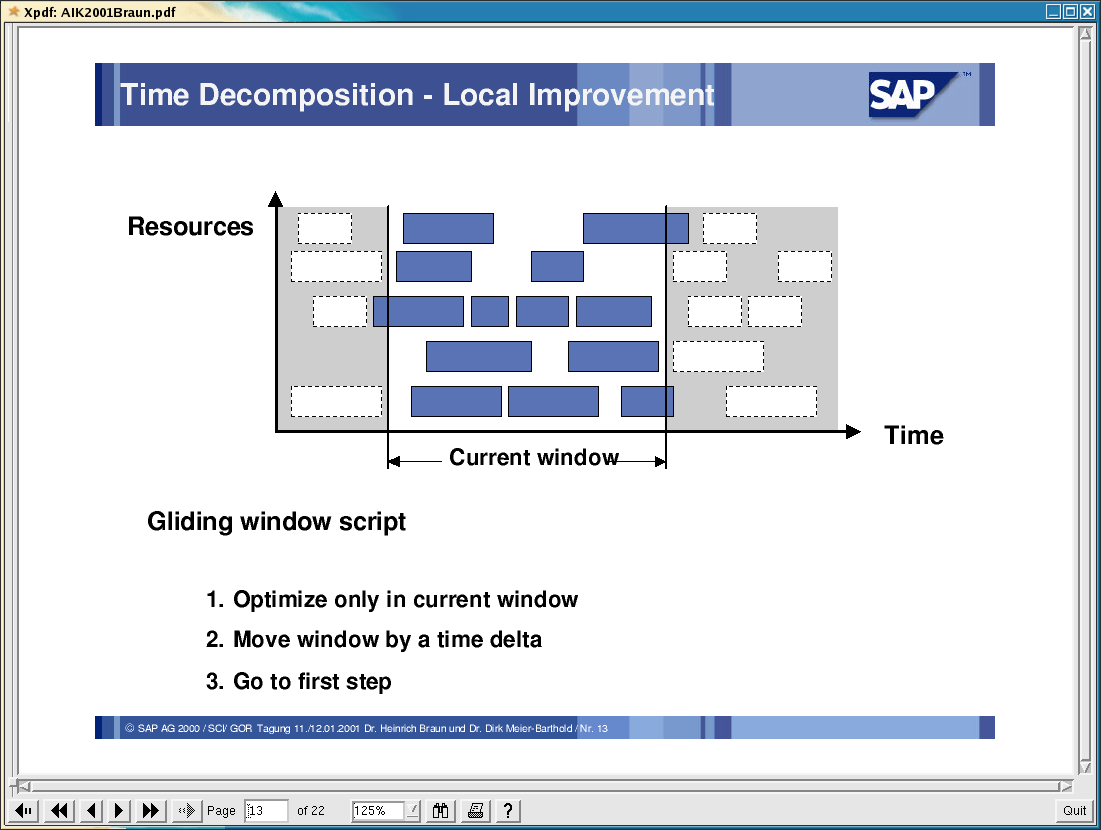
\includegraphics[scale=0.2]{sap1.png} & 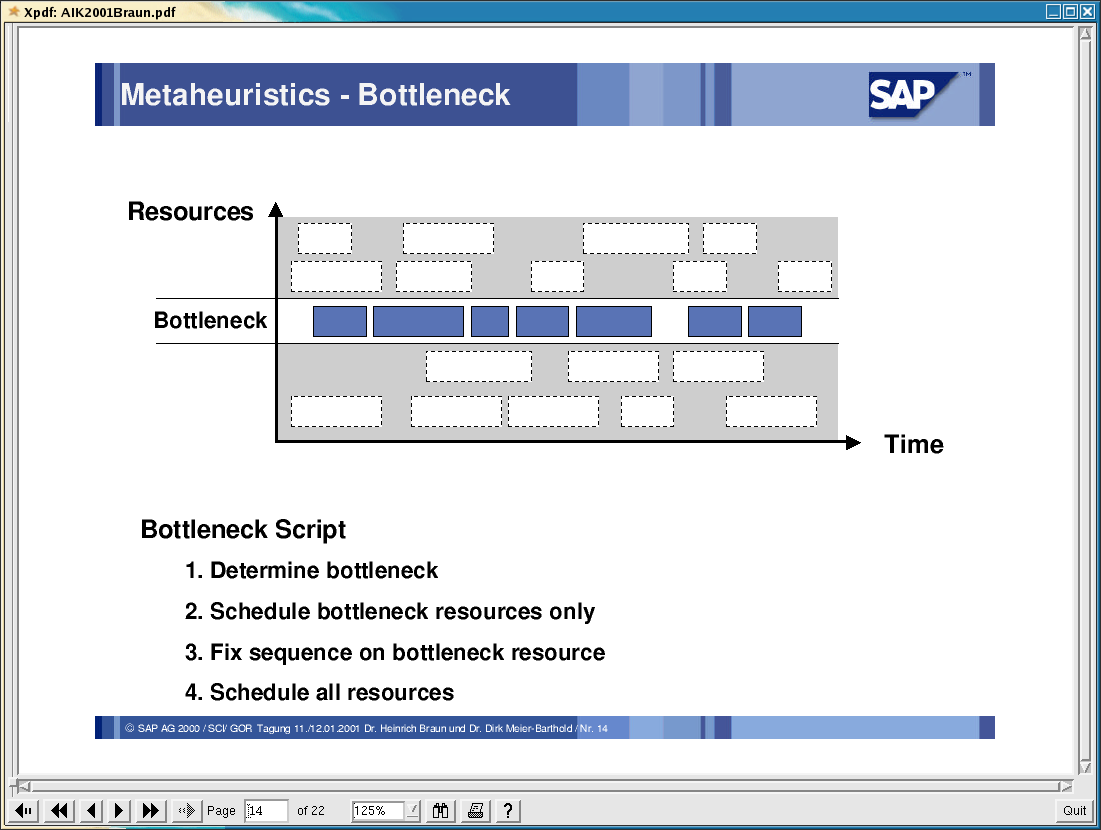
\includegraphics[scale=0.2]{sap2.png}\\
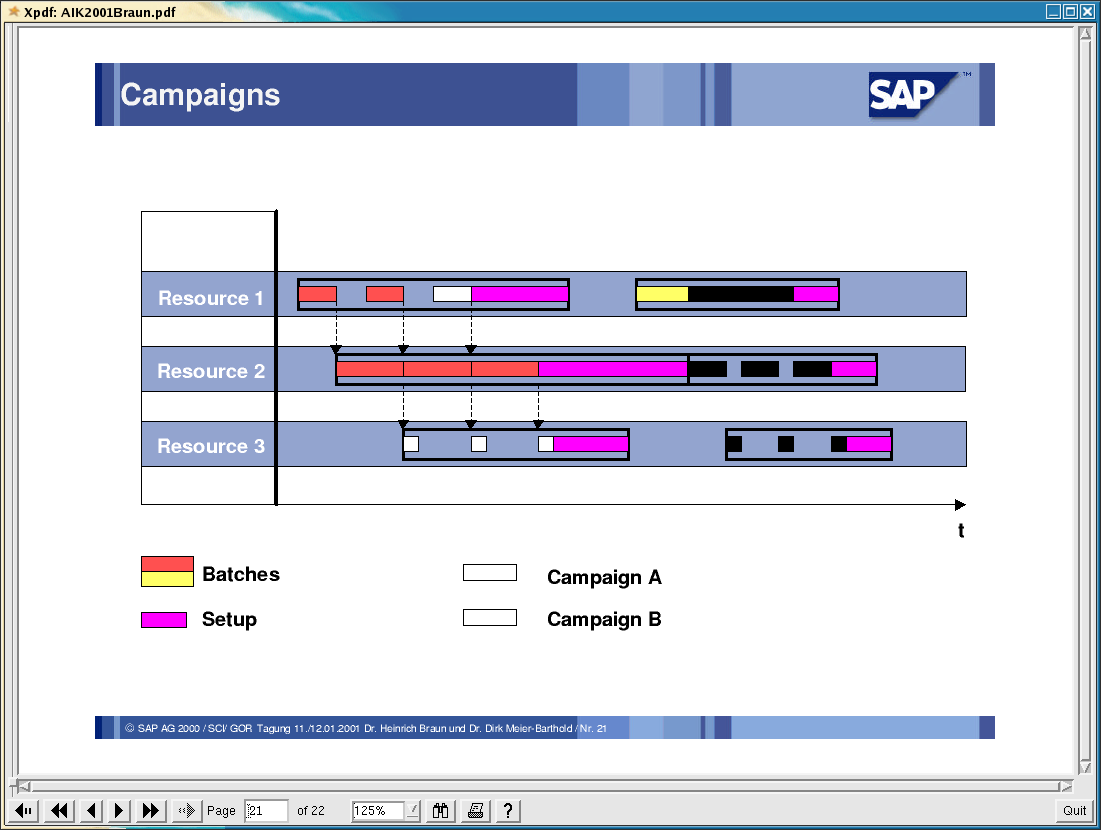
\includegraphics[scale=0.2]{sap3.png} & 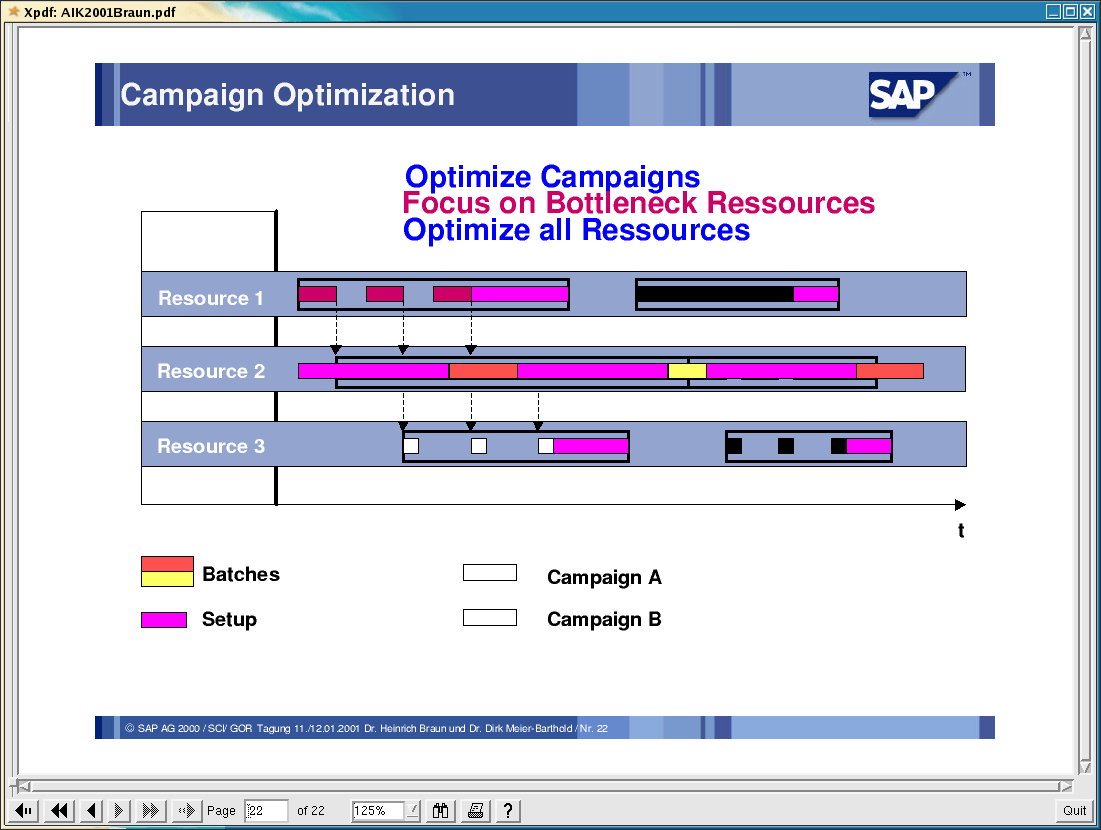
\includegraphics[scale=0.2]{sap4.png}
\end{tabular}
\caption{Beispiel Optimierer von SAP}
\end{figure}

\newpage
Und einem Optimierer f"ur Strategiespiele:
\begin{figure}[h]
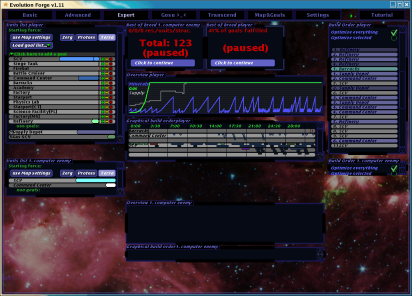
\includegraphics{ef.png} 
\caption{Beispiel Optimierer \textit{Evolution Forge}}
\end{figure}

\begin{thebibliography}{99}
\bibitem{Ross} {\sc Sheldon M. Ross:}  \textit{Introduction to stochastic dynamic programming - Probability and mathematical statistics}, First edition, Academic Press, Inc., 1983
\bibitem{SAP} {\sc Dr. Heinrich Braun:}  \textit{Evolution"are Algorithmen im SAP Supply Chain Management}, http://www.aifb.uni-karlsruhe.de/AIK/aik\_07/AIK2001Braun.pdf
\bibitem{Tandem} {\sc Hyun-Soo Ahn, Izak Duenyas, and Rachel Q. Zhang:} \textit{Optimal Stochastic Scheduling of a 2-Stage Tandem Queue with Parallel Servers}, November, 1997, http://www.ieor.berkeley.edu/~ahn/webstuff/aap.pdf, Seite 16-21
\end{thebibliography}
\end{document}

